\documentclass[a4paper,11pt,fleqn]{article}		% Présentation générale et mise en page


\input{preambule}
\input{preambule-partages}
\input{preambule-axes-gradues}


%\input{preambule}
\setlength{\columnsep}{1cm}
\setlength{\columnseprule}{.5pt}


\renewcommand{\headrulewidth}{1pt}
\fancyhead[C]{\textbf{Entraînement -- Calcul littéral niveau 1 version \no <<version>>}} 
\fancyhead[L]{}
\fancyhead[R]{Cycle 4}

\renewcommand{\footrulewidth}{1pt}
\fancyfoot[C]{} 
\fancyfoot[L]{}
\fancyfoot[R]{Calcul littéral niveau 1}


\usepackage{titlesec}
\titlespacing*{\subsection}
{1pt}{.1ex plus 0.1ex minus .1ex}{.1ex plus .1ex}

\begin{document}

\begin{multicols}{2}

% Il faudrait créer une variable python ["le double","le triple","le quadruple","le quintuple","la moitié",le "tiers","le quart", "le cinquième", "le dixième"] et l'utiliser dans l'exercice ainsi qu'une variable ["la somme", "la différence", "le produit", "le quotient"]
%\exo{}
%
%Traduire par une expression littérale : 
%\begin{enumerate}
%	\item le double de $z$
%	\item le triple de $z$
%	\item la moitié de $z$
%	\item le produit de 7 par $z$
%	\item la somme du produit de 5 par $z$ et du\\ double de $z$
%	\item le double de la somme de 5 et $z$
%\end{enumerate}

\exo{ - Version 1.0}
Quel résultat donne chacun de ces 3 programmes de calculs lorsqu'on prend $x$ comme nombre de départ ?	

\begin{center}
\fcolorbox{black}{gray!30}{
\begin{minipage}{0.7\linewidth}
Programme 1 : 
\begin{itemize}
	\item Multiplier par -7
	\item Ajouter 4
\end{itemize}
\end{minipage}
}

\medskip
\fcolorbox{black}{gray!30}{
\begin{minipage}{0.7\linewidth}
Programme 2 : 
\begin{itemize}
	\item Soustraire -3
	\item Multiplier par -7
\end{itemize}
\end{minipage}
}

\medskip
\fcolorbox{black}{gray!30}{
\begin{minipage}{0.7\linewidth}
Programme 3 : 
\begin{itemize}
	\item Multiplier par 8
	\item Soustraire 2
	\item Prendre le double
\end{itemize}
\end{minipage}
}
\end{center}
\exo{ - Version 2.0}
Quel résultat donne chacun de ces 3 programmes de calculs lorsqu'on prend $x$ comme nombre de départ ?	

\begin{center}
\fcolorbox{black}{gray!30}{
\begin{minipage}{0.7\linewidth}
Programme 1 : 
\begin{itemize}
	\item Multiplier par -5
	\item Ajouter 9
\end{itemize}
\end{minipage}
}

\medskip
\fcolorbox{black}{gray!30}{
\begin{minipage}{0.7\linewidth}
Programme 2 : 
\begin{itemize}
	\item Soustraire 2
	\item Multiplier par 9
\end{itemize}
\end{minipage}
}

\medskip
\fcolorbox{black}{gray!30}{
\begin{minipage}{0.7\linewidth}
Programme 3 : 
\begin{itemize}
	\item Multiplier par 2
	\item Soustraire 5
	\item Prendre le double
\end{itemize}
\end{minipage}
}
\end{center}
\exo{ - Version 3.0}
Quel résultat donne chacun de ces 3 programmes de calculs lorsqu'on prend $x$ comme nombre de départ ?	

\begin{center}
\fcolorbox{black}{gray!30}{
\begin{minipage}{0.7\linewidth}
Programme 1 : 
\begin{itemize}
	\item Multiplier par -8
	\item Ajouter 2
\end{itemize}
\end{minipage}
}

\medskip
\fcolorbox{black}{gray!30}{
\begin{minipage}{0.7\linewidth}
Programme 2 : 
\begin{itemize}
	\item Soustraire 2
	\item Multiplier par -7
\end{itemize}
\end{minipage}
}

\medskip
\fcolorbox{black}{gray!30}{
\begin{minipage}{0.7\linewidth}
Programme 3 : 
\begin{itemize}
	\item Multiplier par 2
	\item Soustraire -9
	\item Prendre le double
\end{itemize}
\end{minipage}
}
\end{center}
\exo{ - Version 4.0}
Quel résultat donne chacun de ces 3 programmes de calculs lorsqu'on prend $x$ comme nombre de départ ?	

\begin{center}
\fcolorbox{black}{gray!30}{
\begin{minipage}{0.7\linewidth}
Programme 1 : 
\begin{itemize}
	\item Multiplier par -3
	\item Ajouter -8
\end{itemize}
\end{minipage}
}

\medskip
\fcolorbox{black}{gray!30}{
\begin{minipage}{0.7\linewidth}
Programme 2 : 
\begin{itemize}
	\item Soustraire 2
	\item Multiplier par 2
\end{itemize}
\end{minipage}
}

\medskip
\fcolorbox{black}{gray!30}{
\begin{minipage}{0.7\linewidth}
Programme 3 : 
\begin{itemize}
	\item Multiplier par 4
	\item Soustraire 4
	\item Prendre le double
\end{itemize}
\end{minipage}
}
\end{center}
\exo{ - Version 1.0}

Simplifier les expressions suivantes.

\begin{multicols}{2}
$A=6 x +2 x$\\
$B=x\times (-7) \times x$\\
$C=7\times x +9\times x$\\
$D=7\times x\times 9\times x$\\
$E=2 \times x-3\times (-9) +5 x$\\
$F=7 \times (-5y -9)$\\
$G=2 a\times  a+a\times 2+a\times 1$\\
$H= 3\times x -6x$
\end{multicols}
\exo{ - Version 2.0}

Simplifier les expressions suivantes.

\begin{multicols}{2}
$A=9 x +8 x$\\
$B=x\times 4 \times x$\\
$C=6\times x +3\times x$\\
$D=6\times x\times 3\times x$\\
$E=3 \times x-3\times 9 +7 x$\\
$F=-8 \times (-3y -2)$\\
$G=2 a\times  a+a\times 1+a\times 1$\\
$H= 2\times x -6x$
\end{multicols}
\exo{ - Version 3.0}

Simplifier les expressions suivantes.

\begin{multicols}{2}
$A=9 x +5 x$\\
$B=x\times (-3) \times x$\\
$C=-5\times x -5\times x$\\
$D=-5\times x\times (-5)\times x$\\
$E=-9 \times x+2\times (-7) -9 x$\\
$F=-7 \times (8y +7)$\\
$G=2 a\times  a+a\times 2+a\times 3$\\
$H= 2\times x +8x$
\end{multicols}
\exo{ - Version 4.0}

Simplifier les expressions suivantes.

\begin{multicols}{2}
$A=3 x +6 x$\\
$B=x\times (-8) \times x$\\
$C=3\times x +6\times x$\\
$D=3\times x\times 6\times x$\\
$E=6 \times x+7\times 3 -8 x$\\
$F=9 \times (3y +3)$\\
$G=1 a\times  a+a\times 1+a\times 3$\\
$H= 8\times x +2x$
\end{multicols}
%
%\exo{}
%
%Calculer les expressions suivantes pour $x=0$.
%
%\begin{tasks}[counter-format = {tsk[1].},label-format={\bfseries}](3)
%	\task $0 x$ 
%	\task $x^2$
%	\task $0x  $
%	\task $ 0 (0 x )$
%	\task $ 0   x$
%	\task $x^3$
%\end{tasks}

\exo{ - Version 1.0}

Développer et réduire les expressions suivantes.

\begin{multicols}{2}
$A=  5 (x  -6)$\\
$B= 7 ( 7 x    +4)$\\
$C=y( -2  +2 y)$\\
$D= 2  t(  -2 t -5)$
\end{multicols}

%
%\exo{}
%
%Calculer les expressions suivantes pour $x=0$.
%
%\begin{tasks}[counter-format = {tsk[1].},label-format={\bfseries}](3)
%	\task $0 x$ 
%	\task $x^2$
%	\task $0x  $
%	\task $ 0 (0 x )$
%	\task $ 0   x$
%	\task $x^3$
%\end{tasks}

\exo{ - Version 2.0}

Développer et réduire les expressions suivantes.

\begin{multicols}{2}
$A=  5 (x  +6)$\\
$B= 9 ( 5 x    +2)$\\
$C=y( 3  -4 y)$\\
$D= 2  t(  3 t -7)$
\end{multicols}

%
%\exo{}
%
%Calculer les expressions suivantes pour $x=0$.
%
%\begin{tasks}[counter-format = {tsk[1].},label-format={\bfseries}](3)
%	\task $0 x$ 
%	\task $x^2$
%	\task $0x  $
%	\task $ 0 (0 x )$
%	\task $ 0   x$
%	\task $x^3$
%\end{tasks}

\exo{ - Version 3.0}

Développer et réduire les expressions suivantes.

\begin{multicols}{2}
$A=  -2 (x  -3)$\\
$B= -2 ( -8 x    -3)$\\
$C=y( -2  +8 y)$\\
$D= 2  t(  -3 t -2)$
\end{multicols}

%
%\exo{}
%
%Calculer les expressions suivantes pour $x=0$.
%
%\begin{tasks}[counter-format = {tsk[1].},label-format={\bfseries}](3)
%	\task $0 x$ 
%	\task $x^2$
%	\task $0x  $
%	\task $ 0 (0 x )$
%	\task $ 0   x$
%	\task $x^3$
%\end{tasks}

\exo{ - Version 4.0}

Développer et réduire les expressions suivantes.

\begin{multicols}{2}
$A=  -7 (x  +5)$\\
$B= -2 ( 8 x    +3)$\\
$C=y( 2  +7 y)$\\
$D= 3  t(  8 t +4)$
\end{multicols}

\exo{ - Version 1.0}

Factoriser les expressions suivantes.

\begin{multicols}{2}
$E=  42 x  -6$\\
$F=  -18 x  +6 x$\\
$G=  -2 x  +2 x^2$\\
$H=  -3 x^2  -9 x^2$
\end{multicols}

\exo{ - Version 2.0}

Factoriser les expressions suivantes.

\begin{multicols}{2}
$E=  27 x  +9$\\
$F=  42 x  +7 x$\\
$G=  -36 x  +9 x^2$\\
$H=  -2 x^2  +3 x^2$
\end{multicols}

\exo{ - Version 3.0}

Factoriser les expressions suivantes.

\begin{multicols}{2}
$E=  81 x  -9$\\
$F=  24 x  +4 x$\\
$G=  -3 x  +3 x^2$\\
$H=  3 x^2  +6 x^2$
\end{multicols}

\exo{ - Version 4.0}

Factoriser les expressions suivantes.

\begin{multicols}{2}
$E=  24 x  +3$\\
$F=  -35 x  +5 x$\\
$G=  32 x  +8 x^2$\\
$H=  5 x^2  +8 x^2$
\end{multicols}

\raggedcolumns
\end{multicols}

\exon{}

\begin{minipage}{0.4\linewidth}
	\begin{center}
	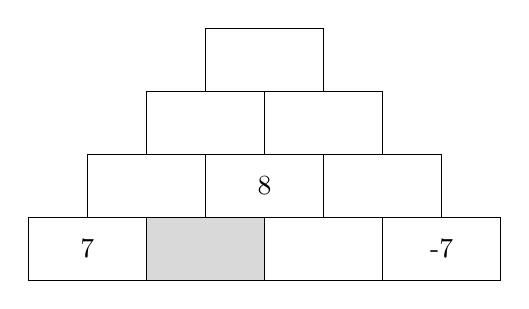
\begin{tikzpicture}
		\tikzstyle{brique}=[minimum width=1.5cm, minimum height=0.8cm,draw]
		\tikzstyle{brique_grise}=[minimum width=1.5cm, minimum height=0.8cm,draw,fill=gray!30]
		\node[brique] at (0,0) {  7 }; % gauche
		\node[brique_grise] at (1.5,0) {};
		\node[brique] at (3,0) {};
		\node[brique] at (4.5,0) { -7 };  % droite
		\node[brique] at (.75,.8) {};
		\node[brique] at (2.25,.8) {  8 };  % milieu bas
		\node[brique] at (3.75,.8) {};
		\node[brique] at (1.5,1.6) {};
		\node[brique] at (3,1.6) {};
		\node[brique] at (2.25,2.4) {};
	\end{tikzpicture} 	
\end{center}
\end{minipage}
\begin{minipage}{0.6\linewidth}
Pour compléter cette pyramide, le nombre situé dans une case est la somme des deux nombres situés en dessous de lui.

\begin{enumerate}
	\item Compléter cette pyramide en mettant un nombre au choix dans la case grise.
	\item Benjamin affirme : \og{} Quel que soit le nombre que je place dans la case grise, je trouve toujours 24 dans la case la plus haute. \fg{}. Est-ce vrai ou faux ? Démontrer le.
\end{enumerate}
\end{minipage}


%\exon{}
%
%
%\begin{center}
%\fcolorbox{black}{gray!30}{
%\begin{minipage}{0.5\linewidth}
%\begin{itemize}
%	\item Multiplier par -8
%	\item Enlever -8
%	\item Multiplier par -8
%	\item Ajouter -8
%	\item Enlever quatre fois le nombre de départ
%\end{itemize}
%\end{minipage}
%}
%\end{center}
%
%\begin{enumerate}
%	\item Après avoir lu ce programme, Benjamin dit : \og{} C'est complètement inutile de faire toutes ces étapes, en un seul calcul je trouve le résultat. \fg{}.\\
%Démontrer que Benjamin a raison et expliquer la seule étape nécessaire.
%	\item Quel nombre de départ faut-il choisir pour obtenir 13 comme résultat avec ce programme de calcul ?
%\end{enumerate}
%
%\exon{}
%
%\begin{tabularx}{\linewidth}{*{4}{>{\centering\arraybackslash}X}}
%\begin{tikzpicture}
%	\tikzstyle{carré}=[minimum width=.5cm, minimum height=.5cm,draw]
%	\node[carré] at (0,0) {};
%\end{tikzpicture}
%&
%\begin{tikzpicture}
%	\tikzstyle{carré}=[minimum width=.5cm, minimum height=.5cm,draw]
%	\node[carré] at (0,0) {};
%	\node[carré] at (-.5,0) {};
%	\node[carré] at (.5,0) {};
%	\node[carré] at (0,.5) {};
%\end{tikzpicture}
%&
%\begin{tikzpicture}
%	\tikzstyle{carré}=[minimum width=.5cm, minimum height=.5cm,draw]
%	\node[carré] at (0,0) {};
%	\node[carré] at (-.5,0) {};
%	\node[carré] at (-1,0) {};
%	\node[carré] at (.5,0) {};
%	\node[carré] at (1,0) {};
%	\node[carré] at (0,.5) {};
%	\node[carré] at (0,1) {};
%\end{tikzpicture}
%&
%\begin{tikzpicture}
%	\tikzstyle{carré}=[minimum width=.5cm, minimum height=.5cm,draw]
%	\node[carré] at (0,0) {};
%	\node[carré] at (-.5,0) {};
%	\node[carré] at (-1,0) {};
%	\node[carré] at (-1.5,0) {};
%	\node[carré] at (.5,0) {};
%	\node[carré] at (1,0) {};
%	\node[carré] at (1.5,0) {};
%	\node[carré] at (0,.5) {};
%	\node[carré] at (0,1) {};
%	\node[carré] at (0,1.5) {};
%\end{tikzpicture}
%\\[-.1cm]
%\textbf{Étape 1} & \textbf{Étape 2} & \textbf{Étape 3} & \textbf{Étape 4}\\
%\end{tabularx}
%
%\bigskip
%\begin{enumerate}
%    \item Combien faut-il de carrés à l'étape 5 ?
%    \item Proposer une formule permettant de calculer le nombre de
%      carrés nécessaires pour l'étape $N$.
%    \item Combien faut-il de carrés à l'étape 1~000 ?
%\end{enumerate}


%	
%
%
%
%\setcounter{exo}{0}
%\vfill
%\begin{correction}
%\begin{multicols}{2}

%
%\exo{}
%
%Programme 1 : $-7 x +4$\\
%Programme 2 : $(x -3)\times (-7)= -7  x  +21 $\\
%Programme 3 : $( 8 x +2 )\times 2= 16 x +2$
%
%\exo{}
%
%
%\begin{multicols}{2}
%$A=0 x$\\
%$B=1x^2$\\
%$C=(7 +9)\times x = 16  x$\\
%$D=7 \times 9\times x^2 = 63\times x^2$\\
%$E=2 \times x -3\times (-9) +5 x$\\
%$F=7 \times (y\times (-5) -9 \times 0)$\\
%$G=2 a\times  a+a\times 2+a\times 1$\\
%$H= 3\times x -6$
%\end{multicols}
%
%
%
%\exo{}
%
%
%\begin{tasks}[counter-format = {tsk[1].},label-format={\bfseries}](3)
%	\task $2\times3=6$ 
%	\task $3^2=9$
%	\task $2\times3-5=1$
%	\task $3\times13=39$
%	\task $2-3=-1$
%	\task $3^3=27$
%\end{tasks}
%
%\exo{}
%
%
%\begin{multicols}{2}
%$A=3x+15$\\
%$B=10x-15$\\
%$C=3y+5y^2$\\
%$D=6t^2-12t$
%\end{multicols}
%
%\end{multicols}
%
%	
%
%
%	
%\end{correction}
\end{document}